\newpage
\section{Frontend}
\label{sec:frontend}


Vector instructions are dispatched to the VFU at an early stage in the host core's pipeline.
These instructions must be dispatched along with updated values of \texttt{vtype} and \texttt{vl}, to control the fault-checking mechanisms.
The \textbf{pipelined fault checker (PFC)} and \textbf{iterative fault checker (IFC)} units perform memory translation for vector memory instructions, and either validate the absence of a memory access-related fault or generate a precise fault ahead of the commit point in the host core.
Instructions validated to be free of faults are dispatched to the VLSU and VU.

\subsection{Core Integration}

Saturn currently supports integration into either Rocket or Shuttle as the host scalar RISC-V core.
The host cores are responsible for decoding vector instructions that must be dispatched to the VFU, in addition to updating and supplying the \texttt{vtype} and \texttt{vl} CSRs to these instructions.

Rocket and Shuttle expose nearly identical interfaces to the vector unit.
The scalar pipeline dispatches vector instructions to the VFU pipeline at the X stage, immediately after scalar operands are read from the scalar register files.
The scalar pipeline also must provide these instructions with up-to-date values of \texttt{vtype}, \texttt{vl}, and \texttt{vstart}.
The M stage exposes a port through which the VFU can access the host core's TLB and MMU.
The WB stage contains interfaces for synchronizing committing or faulting vector instructions with the scalar core's instruction scheme and stalling scalar instruction commit if necessary.
The WB stage also exposes interfaces for modifying \texttt{vstart} and \texttt{vconfig} as vector instructions commit.

\subsubsection{Rocket}

\begin{figure}[h]
  \centering
  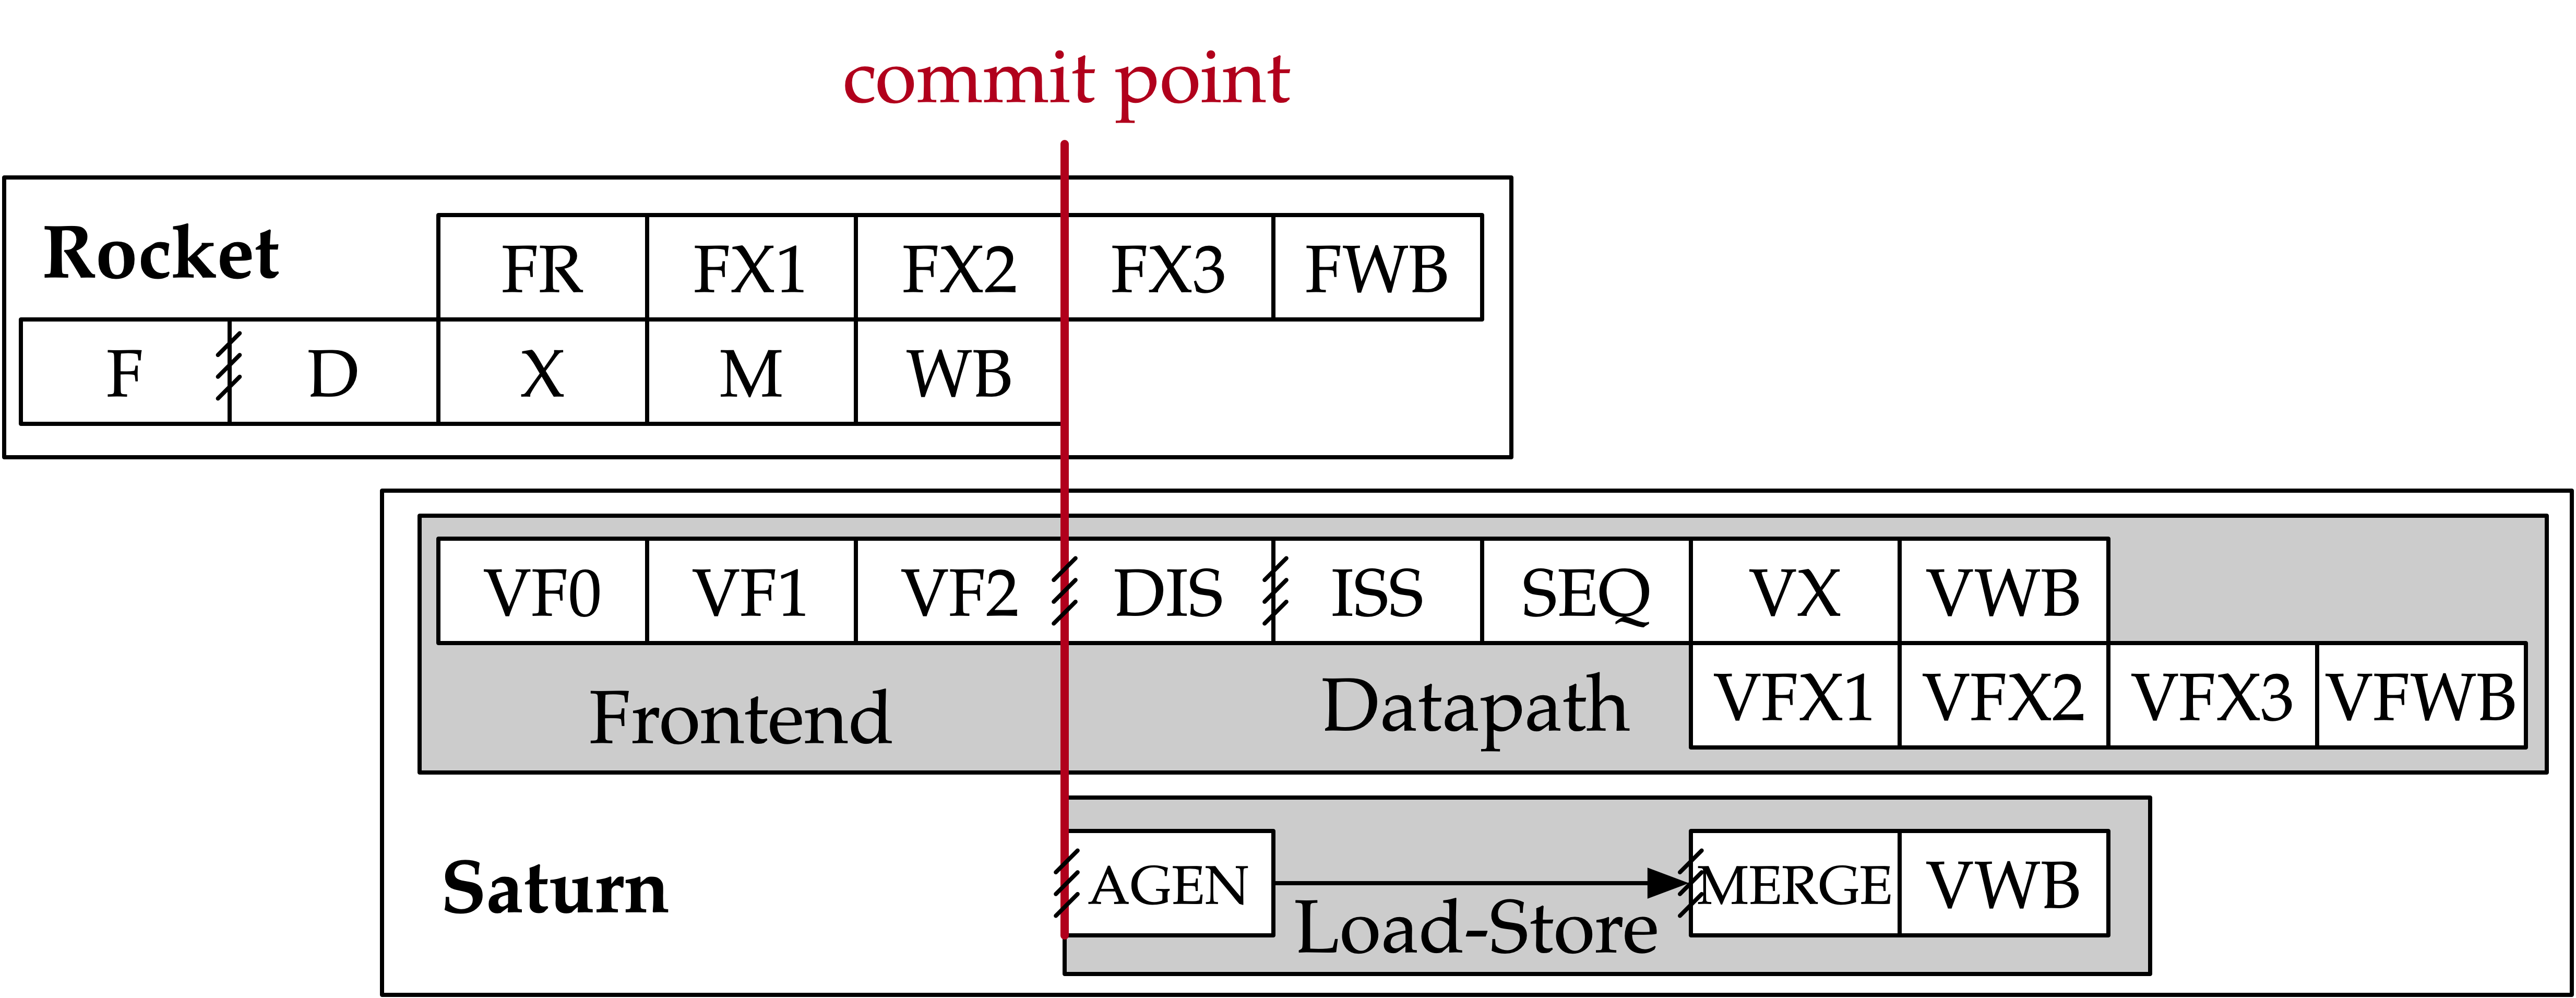
\includegraphics[scale=0.5]{rocketpipe.png}
  \caption{Rocket's pipeline stages with Saturn attached. Hatched lines indicate FIFO queues between pipeline stages.}
  \label{fig:rocket}
\end{figure}

Rocket is a 5-stage in-order single-issue core.
As shown in Figure \ref{fig:rocket}, the Saturn VFU integrates into the execute, memory, and write-back stages of Rocket, where the write-back stage is the commit point.
At the write-back stage, vector instructions which cannot retire due to ongoing activity in the IFC can kill all younger instructions in the earlier pipeline stages, and request the core to re-fetch and replay the instruction at the next PC.
Vector instructions which cannot pass the PFC due to a TLB miss or a lack of capacity in the backend instruction queues are replayed through Rocket's existing replay mechanisms.

\begin{figure}[h]
  \centering
  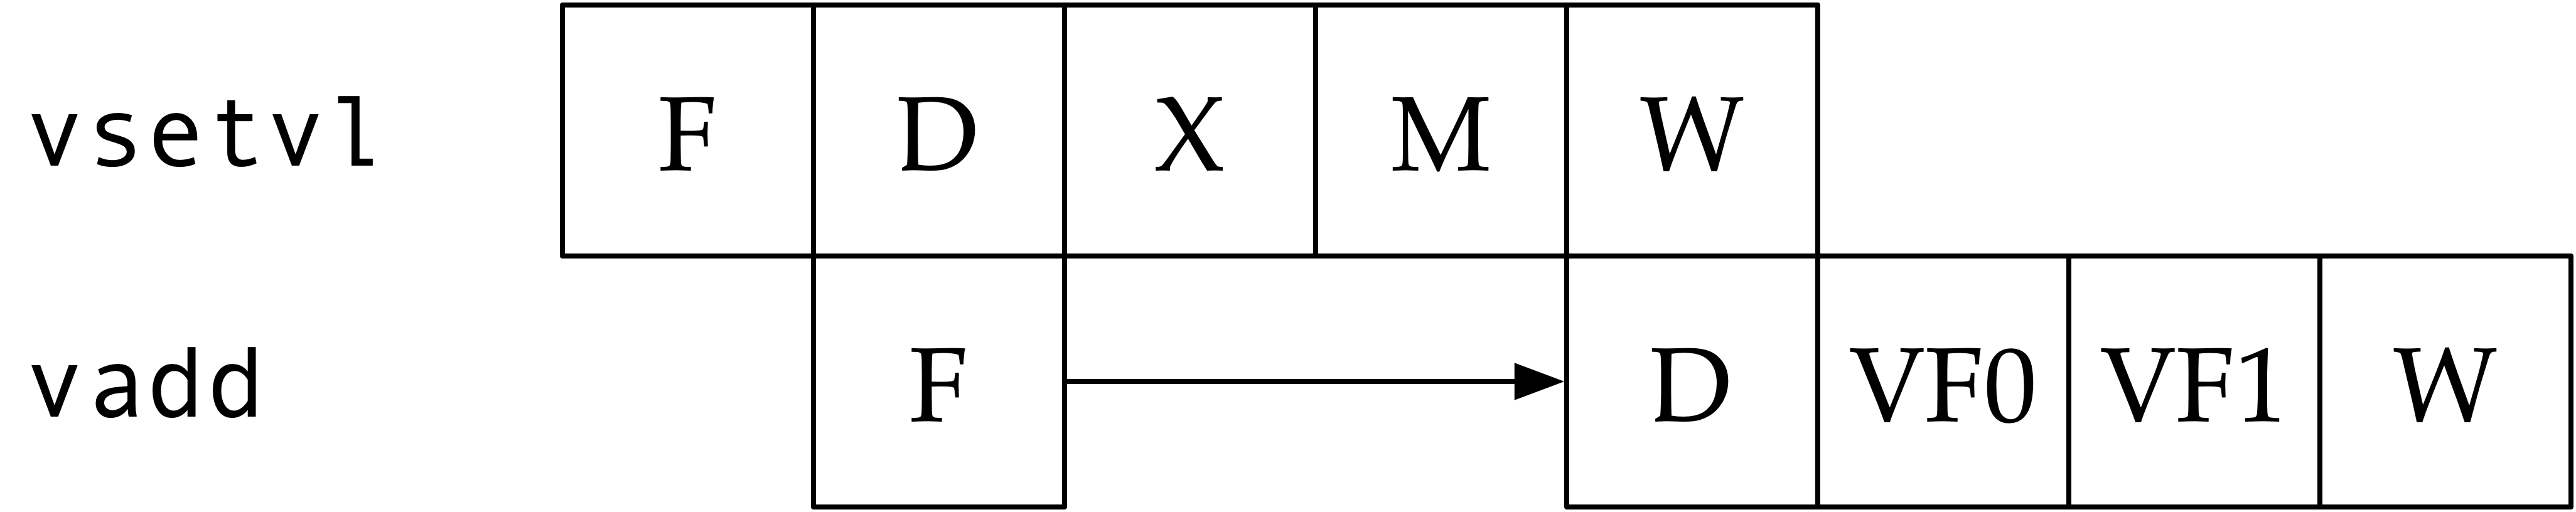
\includegraphics[scale=0.5]{rocketvset.png}
  \caption{\texttt{vset}-induced bubble in Rocket.}
  \label{fig:rocket-vset}
\end{figure}

Rocket does not maintain a speculative copy of the \texttt{vtype} and \texttt{vl} CSRs at the decode stage, so a data hazard can interlock the decode stage whenever a vector instruction proceeds a \texttt{vset} instruction.
As shown in Figure \ref{fig:rocket-vset}, a \texttt{vset} will always induce a 2-cycle bubble on a proceeding vector instruction.
The effect of this is most noticeable in short-chime mixed-precision vector code, in which \texttt{vset} instructions are frequent.


\subsubsection{Shuttle}


\begin{figure}[h]
  \centering
  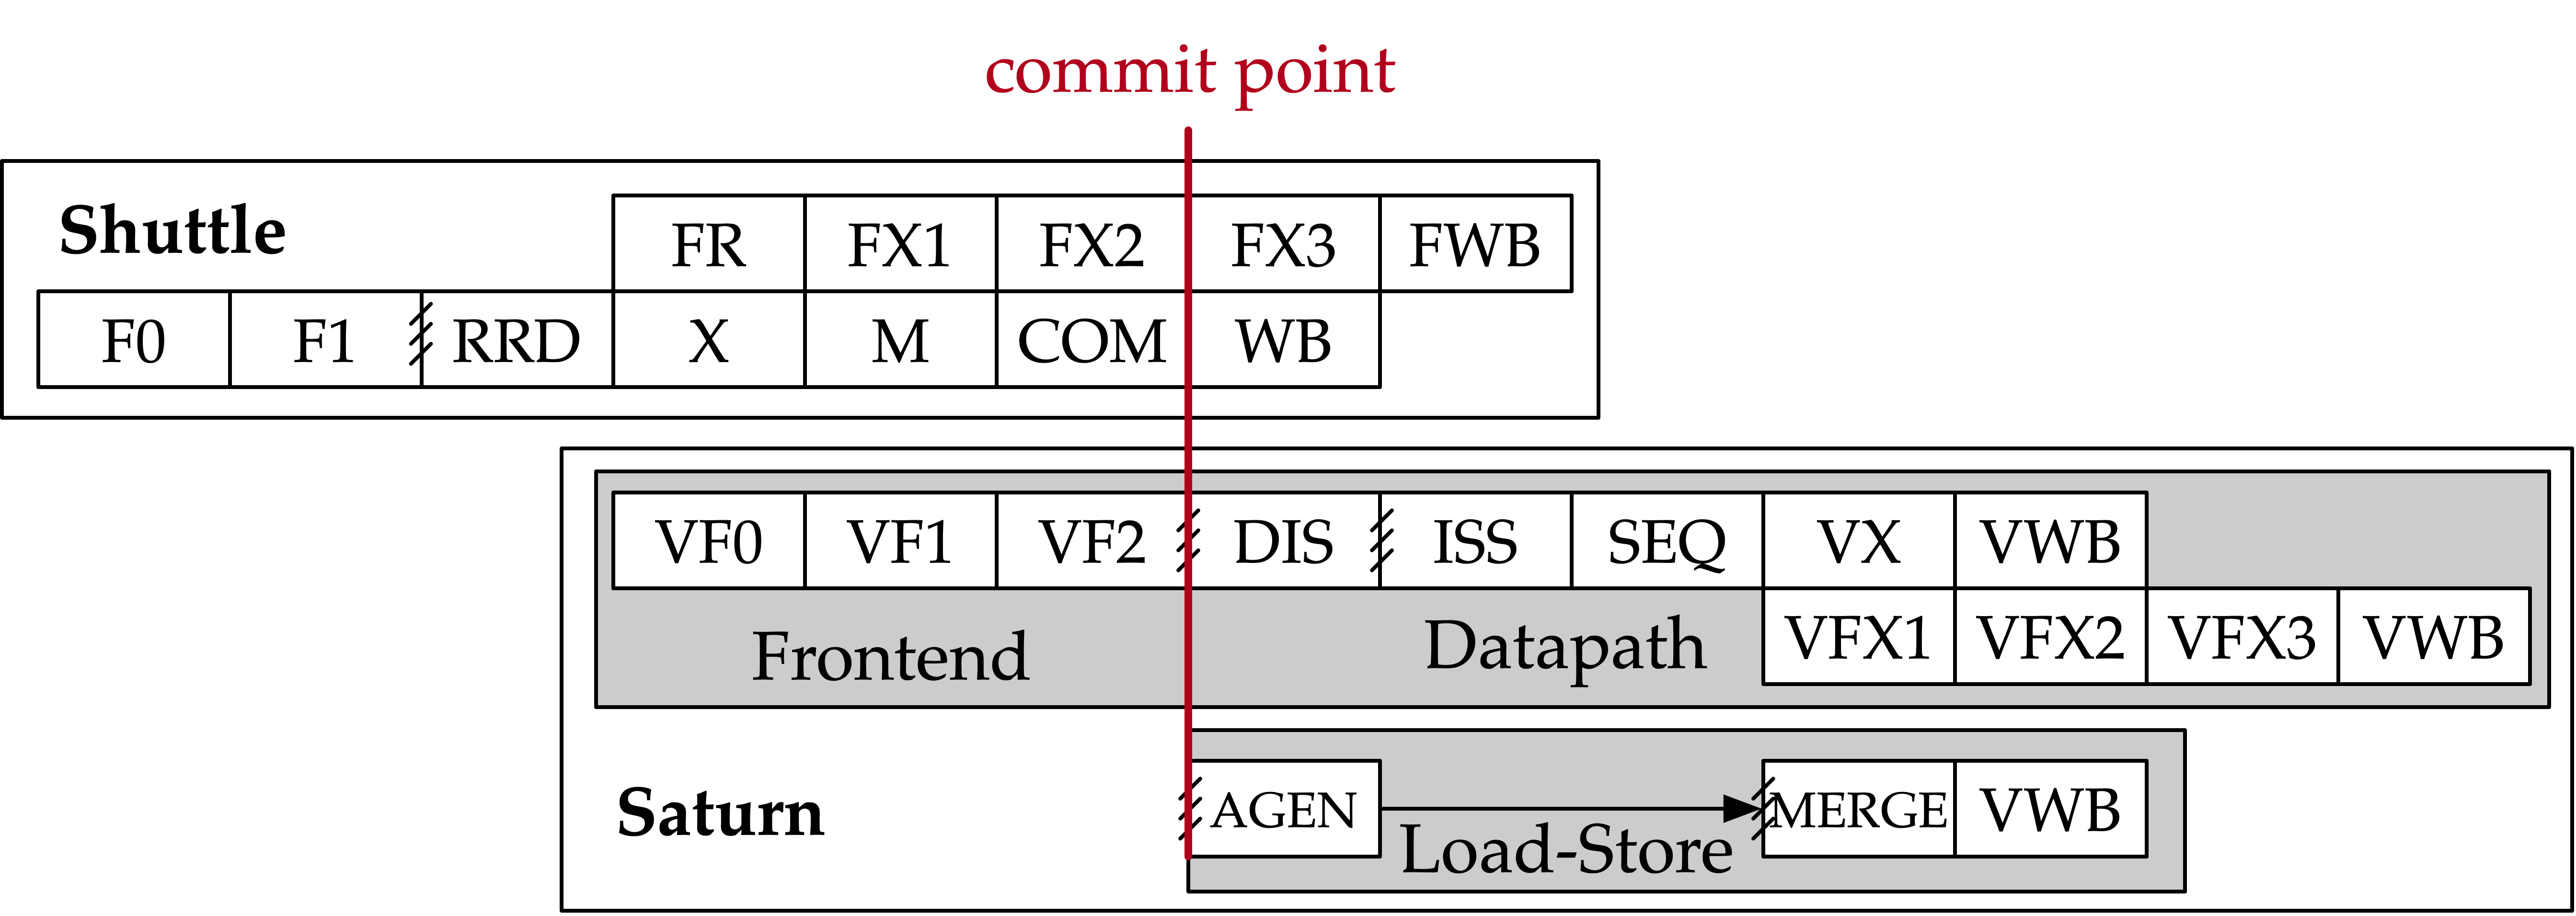
\includegraphics[scale=0.5]{shuttlepipe.png}
  \caption{Shuttle's pipeline stages with Saturn attached. Hatched lines indicate FIFO queues between pipeline stages.}
  \label{fig:shuttle}
\end{figure}


Shuttle is a 7-stage in-order superscalar core, typically configured as 2-issue or 3-issue.
The Saturn VFU integrates into the execute, memory, and commit stages of Shuttle.

Only one of the execution pipes in Shuttle can dispatch into the VFU, but any of the pipes can execute a \texttt{vset} operation.
However, during steady-state operation, Shuttle can dynamically construct instruction packets at the decode stage to maximize instruction throughput given structural hazards by stalling partial instruction packets.

Similar to Rocket, vector instructions that cannot retire at the commit stage will kill younger instructions in the pipeline, and request a refetch and replay of the subsequent instruction.

\begin{figure}[h]
  \centering
  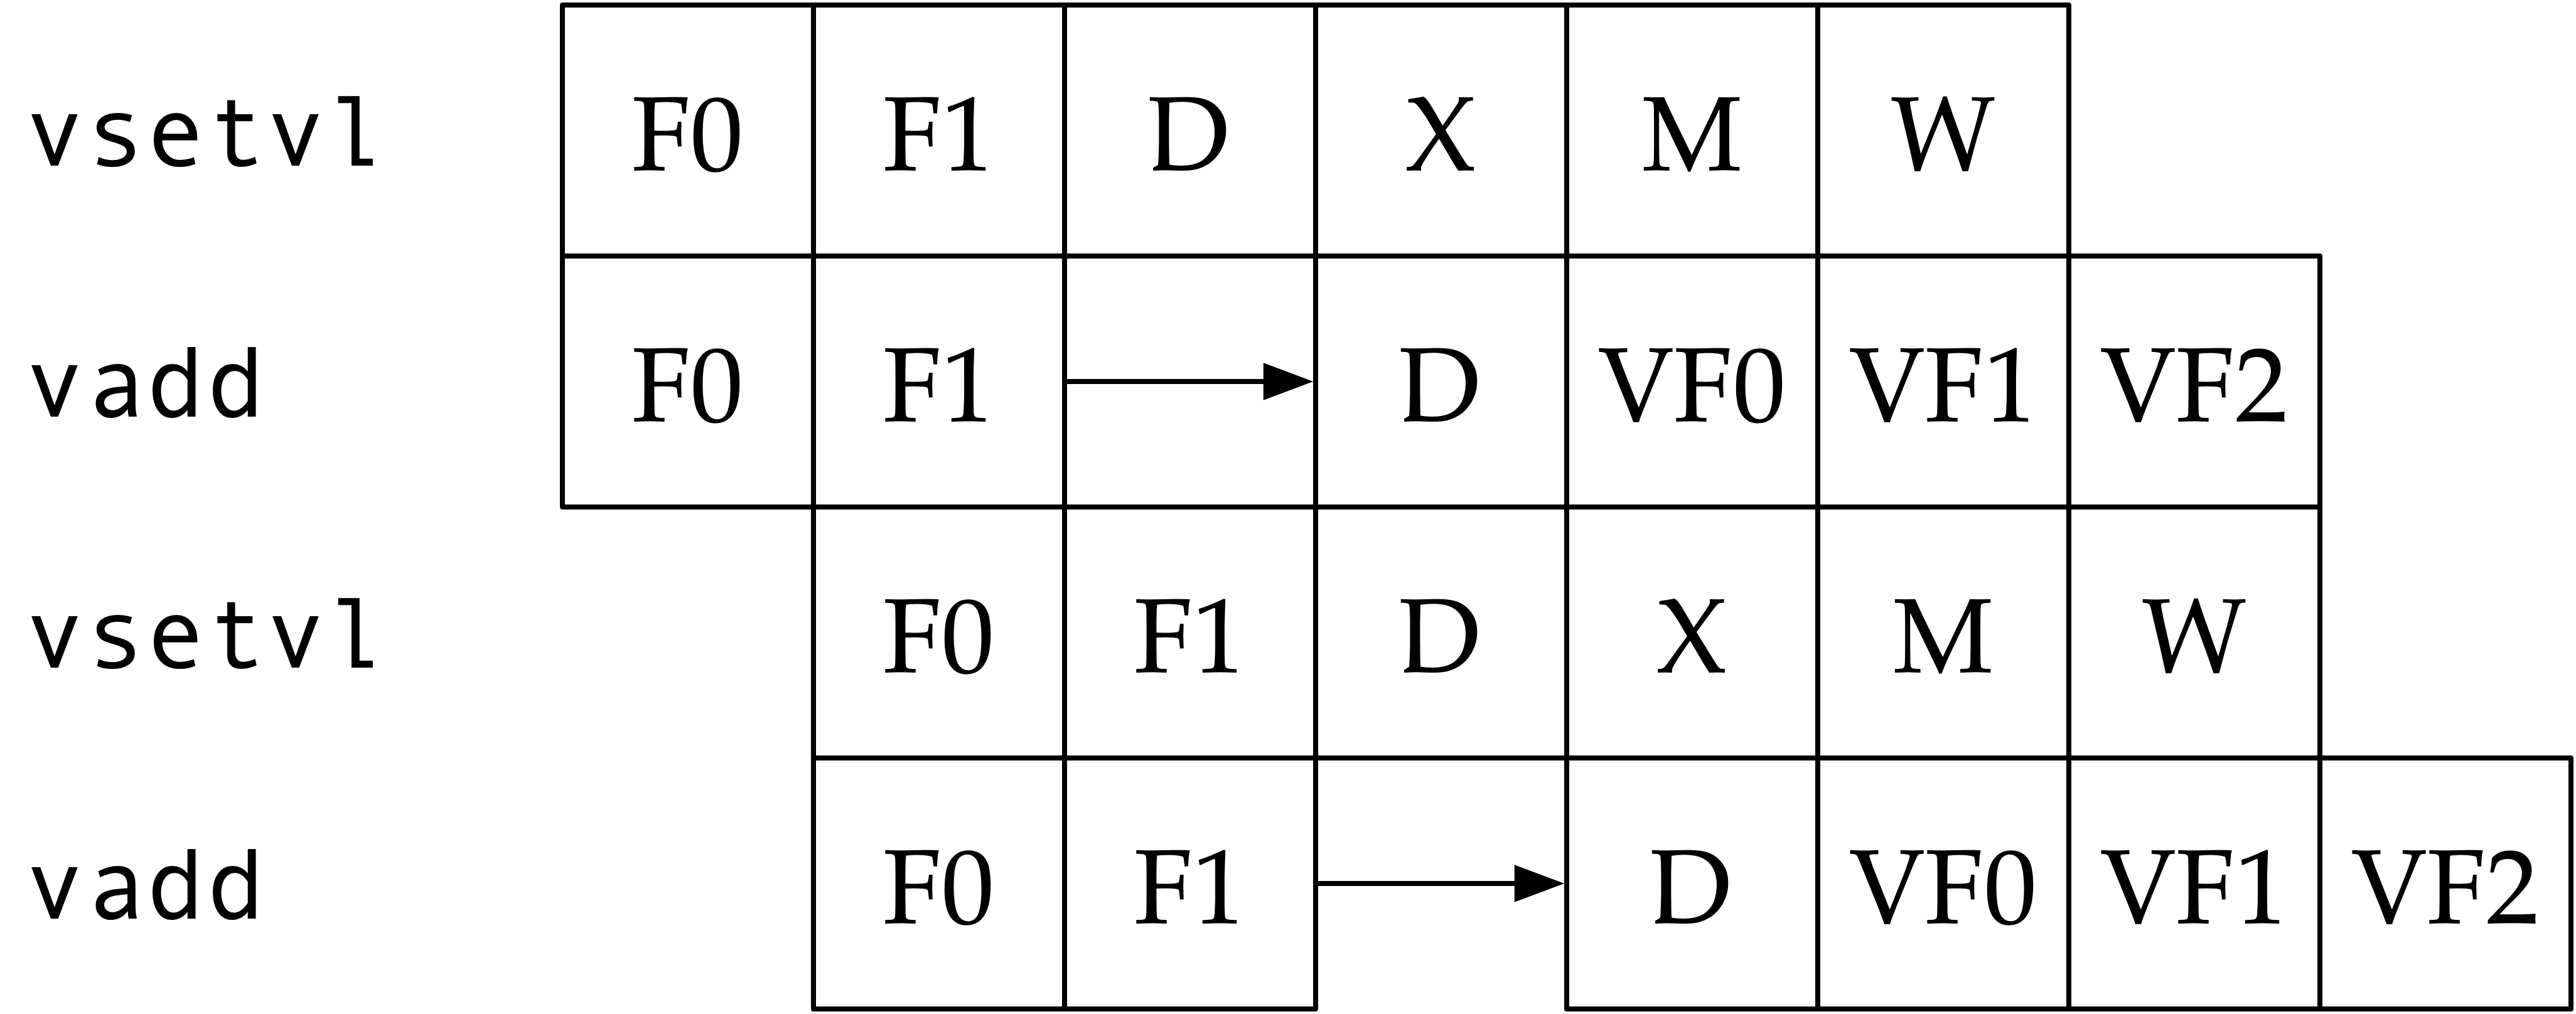
\includegraphics[scale=0.5]{shuttlevset.png}
  \caption{Shuttle dual-issue with forwarding of \texttt{vset}}
  \label{fig:shuttle-vset}
\end{figure}

Unlike Rocket, Shuttle implements a bypass network for \texttt{vset} instructions modifying \texttt{vtype} or \texttt{vl}.
Vector instructions following a \texttt{vset} instruction do not need to stall, as the \texttt{vtype} and \texttt{vl} operands can be accessed through the bypass network.
However, a vector instruction cannot proceed in the same instruction packet as a \texttt{vset}; it must proceed on the next cycle instead.
Figure \ref{fig:shuttle-vset} shows how Shuttle can dynamically stall a partial instruction packet with the \texttt{vadd} to issue it with a younger \texttt{vset} on the next cycle.
This example also depicts how stalling the \texttt{vadd} maintains 2 IPC through Shuttle, and 1 IPC into the vector unit.

\subsection{Memory Translation and Faults}

After entering the VFU, vector instructions first proceed through the pipelined fault checker (PFC).
Instructions that the PFC cannot conservatively guarantee to be free of faults are issued to the IFC.
Instructions that pass the PFC successfully can then be dispatched to the VU and VLSU after they pass the commit point.

Since vector instructions may be speculative ahead of the commit point, any vector instruction flushed by the scalar core is also flushed from the VFU.
The PFC/IFC design pattern achieves the goal of making common case vector instructions fast, through the PFC, while preserving correct precise fault behavior for all vector instructions through the IFC.

The PFC and IFC share access to a single TLB port in the VFU.
This TLB port would typically access the scalar core's TLB.
Future modifications to Saturn could supply a dedicated vector TLB instead.


\subsubsection{Pipelined Fault Checker (PFC)}

The Pipelined Fault Checker is designed to handle common vector instructions without stalling the pipeline at 1 IPC.
Vector instructions fall into one of the following categories:

\begin{itemize}
\item \textbf{Single-page} vector instructions include arithmetic and vector memory instructions for which the extent of the access can be bound to one physical page, at most. This includes unit-strided vector loads and stores that do not cross pages, as well as physically addressed accesses that access a large contiguous physical region. These are the most common vector instructions and need to proceed at high throughput through the VFU.
\item \textbf{Multi-page} vector instructions are memory instructions for which the extent of the instruction's memory access can be easily determined, but the range crosses pages. These are somewhat common vector instructions, and must not incur a substantial penalty.
\item \textbf{Iterative} vector instructions include masked, indexed, or strided memory instructions that might access arbitrarily many pages. These instructions would fundamentally be performance-bound by the single-ported TLB, so the VFU can process these instructions iteratively.
\end{itemize}

In stage-0 (VF0), the PFC establishes which category a vector instruction belongs to.
Note that this does not require memory translation, and can be quickly determined from the instruction opcode, base address offset, and current settings of \texttt{vtype} and \texttt{vl}.

Single-page instructions execute down the PFC pipeline with no stalls.
In stage-1 (VF1), the accessed page is checked through the TLB port.
In stage-2 (VF2), misses in the TLB flush the PFC, forcing the VFU to request a replay of the vector instruction.
This mirrors how the host in-order core handles scalar TLB misses through a replay mechanism.

If the VF2 TLB response indicates an access or page fault, retirement of the instruction is blocked, and the instruction is issued to the IFC to determine if it faults.
This is done because masked vector memory elements that access invalid addresses do not generate faults.
The IFC maintains the capability to access the vector register file for the mask operand, if present.

Page-crossing instructions incur multiple cycles of occupancy in the PFC.
The VF1 stage computes the number of elements within the first page, then updates \texttt{vstart} and requests a replay from the scalar core at the same PC.
The replayed instruction will repeatedly see a non-zero \texttt{vstart}, compute an updated base address at the next page, and request a replay if the remaining elements cross pages, until all the pages have been checked.
In the VF2 stage, the PFC will set the \texttt{vstart} and \texttt{vl} signals for the vector instructions dispatched into the VU and VLSU to correctly set the partial execution of such instructions.
This behavior cracks page-crossing contiguous loads and stores into single-page operations.


\subsubsection{Iterative Fault Checker (IFC)}

Iterative instructions cannot be conservatively bound by the PFC.
Instead, these instructions perform a no-op through the PFC and are issued to the IFC.
Unlike the PFC, which operates page-by-page, the IFC executes element-by-element, requesting index and mask values from the VU for indexed and masked vector operations.
The IFC generates a unique address for each element in the vector access, checks the TLB, and dispatches the element operation for that instruction to the VU and VLSU only if no fault is found.
Upon a fault, the precise element index of the access that generates the fault is known, and all accesses preceding the faulting element would have been dispatched to the VU and VLSU.

The IFC accesses the TLB through the same port as the PFC, with arbitration set to prioritize the IFC, as the IFC will always track older instructions than the PFC.
The IFC also can access the VRF through the VU to fetch index or mask data.


\subsubsection{Towards Performant Indexed or Strided Accesses}

Lane-organized long-vector machines often implement high-radix memory systems with many independent memory access ports, enabling high-throughput address generation and good performance on indexed or strided accesses.
In contrast, DSP cores, whether vector or SIMD, typically are integrated into a more conventional memory system designed around contiguous block accesses.
Saturn's VLSU is designed towards deployment as a DSP system, and thus fundamentally has limited performance on indexed or strided accesses, as it can only generate one element's address per cycle for these instructions.

Thus, the design of the IFC, which can only performe one-element-per-cycle translation, matches the throughput of the VLSU.
Improving the throughput of the IFC does yield some benefits even if the VLSU's address generation is fundamentally restricted.
Younger vector instructions after an indexed or strided access can be aggressively issued to the backend, allowing the backend to overlap their execution with other elementwise loads or stores.

To reduce the cases that fall back to the IFC, the PFC can be extended to consider memory region granularities that are larger than a page.
For instance, superpages in virtual memory can exceed the maximum possible extent of an constrained-index-width indexed access or a bounded-stride strided access.
Similarly, when memory translation is disabled, the extent of contiguous physical memory serves as a large bound as well.


\subsection{Scalar-Vector Memory Disambiguation}
\label{sec:scalar-disambig}

Vector memory instructions architecturally appear to execute sequentially with the scalar loads and stores generated by the same hart.
Scalar stores cannot execute while there is a pending older vector load or store to that same address.
Scalar loads cannot execute while there is a pending older vector load to that same address, as doing so could violate the same-address load-load ordering axiom in RVWMO since the vector and scalar loads access different paths into the memory system.
Section \ref{sec:vector-disambig} discusses the mechanisms for vector-vector memory disambiguation.

The S2 stage of the PFC also receives the physical address of the current in-flight scalar load or store about to commit in the host scalar core's W stage.
This address is checked against the older inflight loads and stores in the VLIQ and VSIQ in the VLSU.
On a match, a replay for the younger scalar load or store is requested.

The VLSU does not access or probe the scalar store buffers.
To avoid RAW or WAW memory hazards against scalar stores in a scalar store buffer, the PFC stalls the dispatch of vector instructions in the S2 stage until the scalar store buffer is empty.
We observe that this requirement has minimal impact on most vector codes, as scalar stores are rare in stripmined loops.

\subsection{Interface to VU and VLSU}

The micro-op presented to the VU and VLSU contains the instruction bits, scalar operands, and current \texttt{vtype}/\texttt{vstart}/\texttt{vl} settings for this instruction.
For memory operations, this bundle also provides the physical page index of the accessed page for this instruction, since the PFC and IFC crack vector memory instructions into single-page accesses.
For segmented instructions where a segment crosses a page, \texttt{segstart} and \texttt{segend} bits are additionally included in the bundle, to indicate which slice of a segment resides in the current page.

